\documentclass{beamer}
%Imports and customization
\usepackage{tikz}
\usepackage{graphicx}
\usepackage{tikz-feynman}
\usepackage{ulem}
\usepackage{colortbl}
\graphicspath{ 
    {./images/}
}

\beamertemplatenavigationsymbolsempty
\setbeamertemplate{sidebar right}{}
\setbeamertemplate{footline}{
    \hfill\usebeamertemplate***{navigation symbols}
    \hspace{1cm}\insertframenumber{}/\inserttotalframenumber
}
\setbeamertemplate{caption}{\raggedright\insertcaption\par}
\setbeamersize{text margin left=4mm,text margin right=4mm} 

\setbeamerfont{itemize/enumerate body}{size=\scriptsize}
\setbeamerfont{itemize/enumerate subbody}{size=\scriptsize}
\setbeamerfont{itemize/enumerate subsubbody}{size=\scriptsize}


%Custom Macros
\newcommand{\statwarn}{
    \tiny \color{red} Absolute numbers here mean NOTHING. Plots are based on small (100k events) samples, and are highly biased. All that matters is relative position!
}


% WARNING: When using these commands, the image argument must
% NOT have spaces between itself and the braces
\newcommand{\fullscreenimage}[2]{
    \frame{
        \frametitle{#1} 
        \begin{figure}
        \includegraphics[height=0.9\textheight,width=\textwidth,keepaspectratio]{#2}
        \end{figure}
    }
}


\newcommand{\importpdf}[3]{
    \frame{
        \begin{columns}\column{\dimexpr\paperwidth-10pt}
        \begin{figure}
        \includegraphics[page=#2,height=0.8\textheight,width=\textwidth,keepaspectratio]{#1}
        \end{figure}

        {\tiny #3}
        \end{columns}
    }
}


\newcommand{\displayone}[3]{
    \frame{
        \frametitle{#1} 
        \begin{columns}
            \begin{column}{0.5\textwidth}
                #2
            \end{column}
            \begin{column}{0.5\textwidth}
                \begin{figure}
                    \includegraphics[width=\linewidth,height=\textheight,keepaspectratio]{#3}
                \end{figure}
            \end{column}
        \end{columns}
    }
}

\newcommand{\displayonelarge}[3]{
    \frame{
        \frametitle{#1} 
        \begin{columns}
            \begin{column}{0.3\textwidth}
                #2
            \end{column}
            \begin{column}{0.7\textwidth}
                \begin{figure}
                    \includegraphics[width=\linewidth,height=0.8\textheight,keepaspectratio]{#3}
                \end{figure}
            \end{column}
        \end{columns}
    }
}


\newcommand{\displaytwo}[4]{
    \frame{
        \frametitle{#1} 
        #2
        \begin{columns}
            \begin{column}{0.5\textwidth}
                \begin{figure}
                    \includegraphics[width=\linewidth,height=\textheight,keepaspectratio]{#3}
                \end{figure}
            \end{column}
            \begin{column}{0.5\textwidth}
                \begin{figure}
                    \includegraphics[width=\linewidth,height=\textheight,keepaspectratio]{#4}
                \end{figure}
            \end{column}
        \end{columns}
    }
}

\newcommand{\displaytwocaption}[6]{
    \frame{
        \frametitle{#1} 
        #2
        \begin{columns}
            \begin{column}{0.5\textwidth}
                \begin{figure}
                    \includegraphics[width=\linewidth,height=\textheight,keepaspectratio]{#3}
                    \caption{#4}
                \end{figure}
            \end{column}
            \begin{column}{0.5\textwidth}
                \begin{figure}
                    \includegraphics[width=\linewidth,height=\textheight,keepaspectratio]{#5}
                    \caption{#6}
                \end{figure}
            \end{column}
        \end{columns}
    }
}

\newcommand{\displaytwoVcaption}[6]{
    \frame{
        \begin{columns}
            \begin{column}{0.5\textwidth}
                \frametitle{#1} 
                #2
            \end{column}
            \begin{column}{0.5\textwidth}
                \begin{figure}
                    \includegraphics[width=\linewidth,height=0.3\textheight,keepaspectratio]{#3}
                    \caption{#4}
                \end{figure}

                \begin{figure}
                    \includegraphics[width=\linewidth,height=0.3\textheight,keepaspectratio]{#5}
                    \caption{#6}
                \end{figure}
            \end{column}
        \end{columns}
    }
}


\newcommand{\displaythree}[5]{
    \frame{
        \begin{columns}[T]
            \begin{column}{0.4\textwidth}
                {\usebeamercolor[fg]{title} \insertframetitle{#1} }\\
                \vspace{5mm}
                #2
            \end{column}
            \begin{column}{0.4\textwidth}
                \begin{figure}
                    \includegraphics[width=\linewidth,height=\textheight,keepaspectratio]{#3}
                \end{figure}
            \end{column}
        \end{columns}
        \begin{columns}[T]
            \begin{column}{0.4\textwidth}
                \begin{figure}
                    \includegraphics[width=\linewidth,height=\textheight,keepaspectratio]{#4}
                \end{figure}
            \end{column}
            \begin{column}{0.4\textwidth}
                \begin{figure}
                    \includegraphics[width=\linewidth,height=\textheight,keepaspectratio]{#5}
                \end{figure}
            \end{column}
        \end{columns}
    }
}


\newcommand{\displayfour}[5]{
    \frame{
        \frametitle{#1} 
        \begin{columns}[T]
            \begin{column}{0.4\textwidth}
                \begin{figure}
                    \includegraphics[width=\linewidth,height=\textheight,keepaspectratio]{#2}
                \end{figure}
            \end{column}
            \begin{column}{0.4\textwidth}
                \begin{figure}
                    \includegraphics[width=\linewidth,height=\textheight,keepaspectratio]{#3}
                \end{figure}
            \end{column}
        \end{columns}
        \begin{columns}[T]
            \begin{column}{0.4\textwidth}
                \begin{figure}
                    \includegraphics[width=\linewidth,height=\textheight,keepaspectratio]{#4}
                \end{figure}
            \end{column}
            \begin{column}{0.4\textwidth}
                \begin{figure}
                    \includegraphics[width=\linewidth,height=\textheight,keepaspectratio]{#5}
                \end{figure}
            \end{column}
        \end{columns}
    }
}


\newcommand{\pstrike}[2]{
    \only<-\the\numexpr#1-1>{#2}
    \only<#1->{\sout{#2}}
}


\newcommand{\announcesection}[1]{
    \section{#1}
    \frame{
        \begin{center}
            {\huge #1} 
        \end{center}
    }
}

\newcommand{\kvv}{\kappa_{2V}}
\newcommand{\kl}{\kappa_{\lambda}}
\newcommand{\kv}{\kappa_{V}}

\newcommand{\fkvv}[1]{\kappa_{2V,#1}}
\newcommand{\fkl} [1]{\kappa_{\lambda,#1}}
\newcommand{\fkv} [1]{\kappa_{V,#1}}

\newcommand{\importpdfwpages}[3]{
    \foreach \pageN in {#2,...,#3}{
        \importpdf{#1}{\pageN}{}
    }
}

\newcommand{\hyper}[2]{{\color{blue}\href{#1}{#2}}}



%Begin Presentation
\begin{document}
    \title{VBF/ggF Discrimination in HH$\rightarrow$4b}
    \author{Chris Milke}
    \institute{Southern Methodist University}
    \date{28 May, 2020}

    \frame{\titlepage}
    \announcesection{Introduction}

% Theory 1: SM
\displayonelarge{The Standard Model of Particle Physics}{
    {\footnotesize
    Description of all (known) matter.
    \vspace{5mm}

    Founded on paradigm (symmetry) which relied on
        principle that ``forces'' can be described
        as interactions mediated by \textit{massless} gauge boson particles.
    \vspace{5mm}

    Confoundingly, the W and Z bosons \textit{do} have mass.
    The cornerstone of the SM is in how it resolves this mass...
        %requiring either a modification to 
        %(or complete overhaul of) the theory.}
    }
}{theory/Standard_Model_of_Elementary_Particles}

% Theory 2: Higgs Field
\displayone{The Higgs Mechanism}{
    The Higgs mechanism posits the existence of a ``Higgs Field''
        which induces mass in any particles it interacts with it.
    \vspace{5mm}

    This field was predicted to manifest in the form of a scalar particle,
        the Higgs boson,
        and was detected in 2012 by the CMS and ATLAS experiments.
    \vspace{5mm}
}{theory/higgspotential}

% VVh, VVHH, HHH, HHHH (backup)
\frame{
    \frametitle{Electroweak-Higgs Interactions}

    Some key properties of the Higgs are still poorly understood,
        but could be probed via di-Higgs production.


    \begin{figure}
    \centering
    \begin{subfigure}{0.32\textwidth} 
        \resizebox{0.9\textwidth}{!}{
\begin{tikzpicture} \begin{feynman}
    \vertex (kv) {$\kv$};
    \vertex [right=of kv] (h) {$h$};
    \vertex [above left=of kv] (vb1) {$V_1$};
    \vertex [below left=of kv] (vb2) {$V_2$};

    \diagram* {
        (vb1) -- [boson] (kv) -- [boson] (vb2),
        (kv) -- [scalar] (h),
    };
\end{feynman} \end{tikzpicture}
}
 
        \caption{$VVh$}
    \end{subfigure}
    \begin{subfigure}{0.32\textwidth}
        \resizebox{0.8\textwidth}{!}{
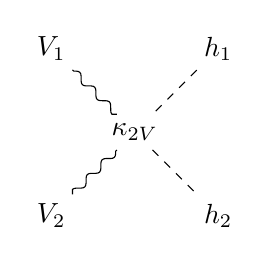
\begin{tikzpicture} \begin{feynman}
    \vertex (k2v) {$\kvv$};
    \vertex [above right=of k2v] (h1) {$h_1$};
    \vertex [below right=of k2v] (h2) {$h_2$};
    \vertex [above left=of k2v] (vb1) {$V_1$};
    \vertex [below left=of k2v] (vb2) {$V_2$};

    \diagram* {
        (vb1) -- [boson] (k2v) -- [boson] (vb2),
        (h1) -- [scalar] (k2v) -- [scalar] (h2),
    };
\end{feynman} \end{tikzpicture}
}
 
        \caption{$VVhh$}
    \end{subfigure}
    \begin{subfigure}{0.32\textwidth}
        \resizebox{0.9\textwidth}{!}{
\begin{tikzpicture} \begin{feynman}
    \vertex (h0) {$h_0$};
    \vertex [right=of h0] (kl) {$\kl$};
    \vertex [above right=of kl] (h1) {$h_1$};
    \vertex [below right=of kl] (h2) {$h_2$};

    \diagram* {
        (h0) -- [scalar] (kl),
        (h1) -- [scalar] (kl) -- [scalar] (h2),
    };
\end{feynman} \end{tikzpicture}
}
 
        \caption{$hhh$}
    \end{subfigure}
    \end{figure}

    The Standard Model predicts how frequently these interactions should occur.
    By providing the conditions necessary for these interactions,
        one can measure how often they actually occur vs their theoretically predicted rate
        (the interactions' ``$kappa$-value'').
}

%% Theory 3: Higgs Lagrangian and its (electroweak) couplings
%\frame{
%    \frametitle{}
%    {\footnotesize
%    \begin{equation} \begin{split} \label{eq:higgskappas}
%        \Lag_h &= \frac{1}{2} \left(\partial^2 - m_h^2 \right) h^2
%            + \kv g_{HVV} V^2 h + \kvv \frac{g_{HHVV}}{2} V^2 h^2
%            + \kl \frac{g_{HHH}}{3!} h^3 + \kappa_{2\lambda} \frac{g_{HHHH}}{4!} h^4
%         \nonumber
%    \end{split} \end{equation}
%    }
%}

% Theory 3: di-Higgs and VBF->HH->bbbb
\frame{
    \frametitle{Vector Boson Fusion, di-Higgs Production, and the All-Hadronic Final State}
    \begin{columns}
        \begin{column}{0.4\textwidth}
            \resizebox{.8\textwidth}{!}{
\begin{tikzpicture} \begin{feynman}
    \vertex (c2v) {???};
    \vertex [above right=of c2v] (h1) {$h_1$};
    \vertex [below right=of c2v] (h2) {$h_2$};
    \vertex [above left=of c2v] (vb1);
    \vertex [below left=of c2v] (vb2);
    \vertex [left=of vb1] (q1) {$q_1$};
    \vertex [left=of vb2] (q2) {$q_2$};
    \vertex [above right=of h1] (b1) {$b$};
    \vertex [below right=of h2] (bbar2) {$\bar b$};
    \vertex [below=of b1] (bbar1) {$\bar b$};
    \vertex [above=of bbar2] (b2) {$b$};

    \vertex [above=of b1] (q3) {$q_3$};
    \vertex [below=of bbar2] (q4) {$q_4$};

    \diagram* {
        (q1) -- (vb1) -- (q3),
        (q2) -- (vb2) -- (q4), 
        (vb1) -- [boson] (c2v) -- [boson] (vb2),
        (h1) -- [scalar] (c2v) -- [scalar] (h2),
        (b1) -- (h1) -- (bbar1),
        (b2) -- (h2) -- (bbar2),
    };
\end{feynman} \end{tikzpicture}
}
 
        \end{column}
        \begin{column}{0.6\textwidth}
            \begin{table}
\centering
\scriptsize
\begin{tabular}{|l|l|l|}
    \hline
    Decay channel & Branching ratio & Rel. uncertainty  \\
    \hline
    $ H \to b \bar{b}        $    & $5.82 \times 10^{-1} $    & $ +1.2\% \atop -1.3\% $ \\
    $ H \to W^+ W^-          $    & $2.14 \times 10^{-1} $    & $\pm 1.5\%        $   \\
    $ H \to \tau^+ \tau^-    $    & $6.27 \times 10^{-2} $    & $\pm 1.6\%        $   \\
    $ H \to c \bar{c}        $    & $2.89 \times 10^{-2} $    & $ +5.5\% \atop -2.0\% $ \\
    $ H \to ZZ               $    & $2.62 \times 10^{-2} $    & $\pm 1.5\%        $   \\
    $ H \to \gamma \gamma    $    & $2.27 \times 10^{-3} $    & $    2.1\%        $   \\
    $ H \to Z \gamma         $    & $1.53 \times 10^{-3} $    & $\pm 5.8\%        $  \\
    $ H \to \mu^+ \mu^-      $    & $2.18 \times 10^{-4} $    & $\pm 1.7\%        $  \\
    \hline
\end{tabular}
\end{table}

        \end{column}
    \end{columns}
}


\frame{
    \frametitle{\hhproc Production}

    \begin{figure}
    \centering
    \begin{subfigure}{0.32\textwidth} 
        \resizebox{0.9\textwidth}{!}{
\begin{tikzpicture} \begin{feynman}
    \vertex (kv1) {$\kv$};
    \vertex [below=of kv1] (kv2) {$\kv$};
    \vertex [right=of kv1] (h1) {$h_1$};
    \vertex [right=of kv2] (h2) {$h_2$};
    \vertex [above left=of kv1] (vb1);
    \vertex [below left=of kv2] (vb2);
    \vertex [left=of vb1] (q1) {$q_{1}$};
    \vertex [left=of vb2] (q2) {$q_{2}$};

    \vertex [above=of h1] (q3) {$q_{3}$};
    \vertex [below=of h2] (q4) {$q_{4}$};

    \diagram* {
        (q1) -- (vb1) -- (q3),
        (q2) -- (vb2) -- (q4), 
        (vb1) -- [boson] (kv1) -- [boson] (kv2)-- [boson] (vb2),
        (h1) -- [scalar] (kv1),
        (h2) -- [scalar] (kv2),
    };
\end{feynman} \end{tikzpicture}
}
 
        \caption{$M_t$}
        \label{fig:tree_level_vbfhh:kv}
    \end{subfigure}
    \begin{subfigure}{0.32\textwidth}
        \resizebox{0.9\textwidth}{!}{
\begin{tikzpicture} \begin{feynman}
    \vertex (kv) {$\kv$};
    \vertex [right=of kv] (kl) {$\kl$};
    \vertex [above right=of kl] (h1) {$h_1$};
    \vertex [below right=of kl] (h2) {$h_2$};
    \vertex [above left=of kv] (vb1);
    \vertex [below left=of kv] (vb2);
    \vertex [left=of vb1] (q1) {$q_{1}$};
    \vertex [left=of vb2] (q2) {$q_{2}$};

    \vertex [above=of h1] (q3) {$q_{3}$};
    \vertex [below=of h2] (q4) {$q_{4}$};

    \diagram* {
        (q1) -- (vb1) -- (q3),
        (q2) -- (vb2) -- (q4), 
        (vb1) -- [boson] (kv) -- [boson] (vb2),
        (kv) -- [scalar] (kl),
        (h1) -- [scalar] (kl) -- [scalar] (h2),
    };
\end{feynman} \end{tikzpicture}
}
 
        \caption{$M_s$}
        \label{fig:tree_level_vbfhh:kl}
    \end{subfigure}
    \begin{subfigure}{0.32\textwidth}
        \resizebox{0.8\textwidth}{!}{
\begin{tikzpicture} \begin{feynman}
    \vertex (k2v) {$\kvv$};
    \vertex [above right=of k2v] (h1) {$h_1$};
    \vertex [below right=of k2v] (h2) {$h_2$};
    \vertex [above left=of k2v] (vb1);
    \vertex [below left=of k2v] (vb2);
    \vertex [left=of vb1] (q1) {$q_{1}$};
    \vertex [left=of vb2] (q2) {$q_{2}$};

    \vertex [above=of h1] (q3) {$q_{3}$};
    \vertex [below=of h2] (q4) {$q_{4}$};

    \diagram* {
        (q1) -- (vb1) -- (q3),
        (q2) -- (vb2) -- (q4), 
        (vb1) -- [boson] (k2v) -- [boson] (vb2),
        (h1) -- [scalar] (k2v) -- [scalar] (h2),
    };
\end{feynman} \end{tikzpicture}
}
 
        \caption{$M_x$}
        \label{fig:tree_level_vbfhh:k2v}
    \end{subfigure}
    \end{figure}

    \begin{equation} \begin{split}
        \sigma &\propto |  \kv^2 M_t + \kv \kl M_s + \kvv M_x |^2 \\
        \sigma &\propto \kv^2 \kl^2 a_1 + \kv^4 a_2 + \kvv^2 a_3 + \kv^3 \kl a_4 + \kv \kl \kvv a_5 + \kv^2 \kvv a_6
    \end{split} \end{equation}
}

% LHC 1: xsec/lumi
\frame{
    \frametitle{Cross-section and Integrated Luminosity}

    {
    \begin{equation} \begin{split}
        \textrm{Expected Events} &= (\textrm{Probability}) \times (\textrm{Number of repeated trials}) \\
        &\downarrow \\
        \textrm{Expected Events} &= \sigma \times L_{\textrm{integrated}}
        \nonumber
    \end{split} \end{equation}
    }
    \vspace{5mm}

    \begin{center}
    \begin{tabular}{ rll }
    $\sigma$ & $\rightarrow$ & Units of cross-sectional area (femto-barns, $fb = 10^{-43} m^2$);\\
        &&Purely a function of theory\\
    \\
    $L_{\textrm{integrated}}$ & $\rightarrow$ & Units of inverse area ($\ifb$);\\
        && Purely a function of experimental setup 
    \end{tabular}
    \end{center}


}

%\displayone{Cross-section and Luminosity}{
%    {\scriptsize
%    \begin{equation} \begin{split}
%        %\frac{\mathcal{P}_{\textrm{hit}}}{\textrm{throw}} &= \frac{\textrm{Area}_{\textrm{object}}}{\textrm{Area}_{\textrm{total}}} \\
%        %\textrm{expected hits} &= \frac{\mathcal{P}_{\textrm{hit}}}{{\textrm{throw}}} \times N_{\textrm{throws}}
%        %N_{\textrm{throws}} &= \frac{N_{\textrm{throws}}}{\Delta t} \times \Delta t \\
%        %\textrm{expected hits} &= \frac{\mathcal{P}_{\textrm{hit}}}{{\textrm{throw}}} \times N_{\textrm{throws}}
%        \frac{\mathcal{P}_{\textrm{hit}}}{\textrm{throw}} &= \frac{\xsec}{\textrm{Area}_{\textrm{total}}} \\
%        \frac{\textrm{expected hits}}{\Delta t} &= \frac{\mathcal{P}_{\textrm{hit}}}{{\textrm{throw}}} \times \frac{\textrm{throws}}{\textrm{\Delta t}} \\
%        \textrm{expected hits} &= \frac{\textrm{expected hits}}{\Delta t} \times {\Delta t}
%        \nonumber
%    \end{split} \end{equation}
%    \vspace{3mm}
%
%    \begin{equation} \begin{split}
%        \dXsec &\propto | M | ^2 \\
%        \xsec &= \int \dXsec d\Omega \\
%        L_{\textrm{instantaneous}} &= \frac{1}{\textrm{Area}_{\textrm{total}}} \times \frac{N_{\textrm{throws}}}{\Delta t} \\
%        L_{\textrm{integrated}} &= \int L_{\textrm{instantaneous}} dt \\
%        \textrm{expected events} &= \xsec \times L_{\textrm{integrated}}
%        \nonumber
%    \end{split} \end{equation}
%    }
%}{introduction/xsec_ball}

%\frame{
%    \frametitle{Cross-section and Luminosity}
%    \begin{columns}
%        \begin{column}{0.4\textwidth}
%        \end{column}
%        \begin{column}{0.6\textwidth}
%
%        \end{column}
%    \end{columns}
%}

% LHC 1: overview
\displaytwoV{The Large Hadron Collider}{
    \vspace{10mm}
    \begin{itemize}
        \item Constructed 1995-2007
        \item On border of Switzerland and France
        \item 50-175 meters underground
        \item 26.7 km radius 
        \item 13 TeV center-of-mass collision energy
        \item 139 \ifb of data delivered to Point 1 (126 are used for my analysis)
    \end{itemize}
}{introduction/lhc}{introduction/lhc_pipe}


% ATLAS 1: overview
\displayonelarge{The ATLAS Experiment}{
    {\small
    Massive particle detector array,
        forming a high hermetic, (nearly) $4\pi$ 3D ``camera'' around the particle interaction region
    \vspace{8mm}

    Different subsytems have different roles:
    \begin{itemize}
        \item Tracker = momentum of charged particles
        \item Calorimeter = energy
        \item Muon System = N/A
    \end{itemize}
    }
}{atlas/atlas_xsec}

    \section{Initial Studies}
\fullscreenimage{Comparing Selection Performance}{roc_explanation}
\fullscreenimage{Current Selection Method Performance}{rocs/rocs_initial}

\displayonelarge{Baseline BDT}{
    As a baseline, train BDT with same inputs as current algorithm. It should perform at least as well.
}{rocs/rocs_bdt1}

\displayfour{Fox-Wolfram Moments}
{fw_moments/fox-wolfram_1}
{fw_moments/fox-wolfram_2}
{fw_moments/fox-wolfram_3}
{fw_moments/fox-wolfram_4}


\displaytwo{BDT with Fox-Wolfram Moments}{
    Improvent from first seven FW Moments is minor, but noticeable.
}{rocs/rocs_bdt2}{rocs/rocs_bdt2_zoom}

    % 9 FW moment description (thanks Rachel!) *
    \section{More Sophisticated Techniques}
\frame{
    \frametitle{Exploring Multi-Jet Discriminants: Centrality}
    \begin{columns}
        \begin{column}{0.5\textwidth}
            {\small The VBF initial scatter quark jets are not always the only thing present in VBF events.
            Radiated Jets (ISR \& FSR) are not uncommon, and provide additional handles for analysis.}
            \begin{figure}
                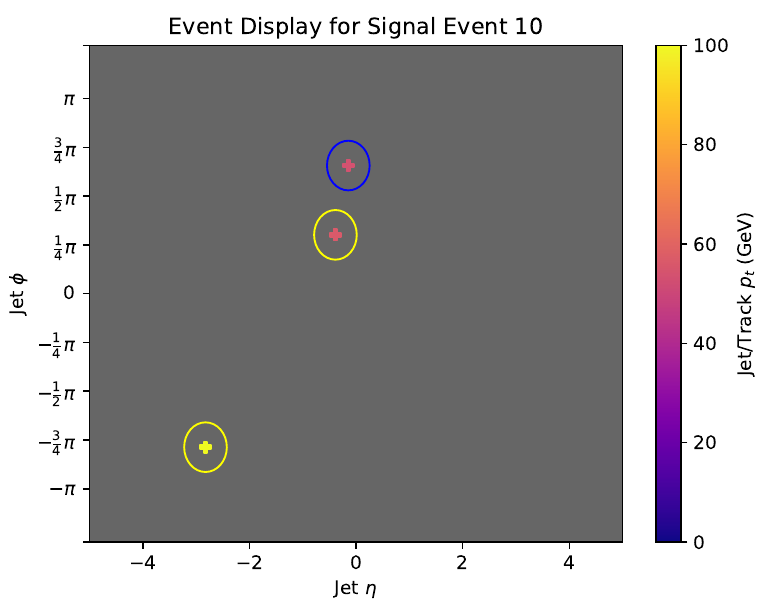
\includegraphics[width=\linewidth,height=\textheight,keepaspectratio]{ event_display}
            \end{figure}
        \end{column}
        \begin{column}{0.5\textwidth}
            \begin{center}\resizebox{0.40\textheight}{!}{ 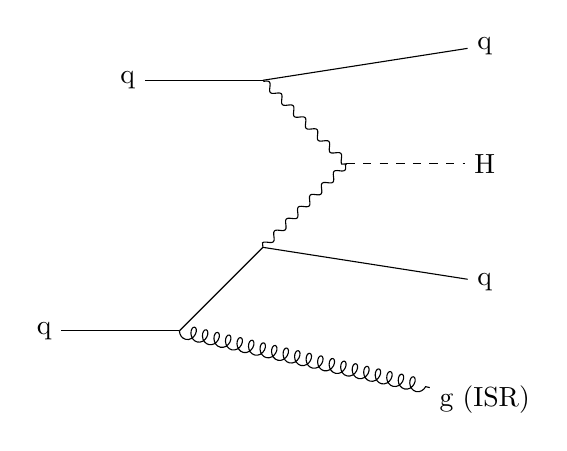
\begin{tikzpicture} \begin{feynman}
    \vertex (a);
    \vertex [right=of a] (b) {H};
    \vertex [above left=of a] (vb1);
    \vertex [below left=of a] (vb2);
    \vertex [left=of vb1] (q1i) {q};
    \vertex [below left=of vb2] (q2k);
    \vertex [left=of q2k] (q2i) {q};
    \vertex [above =of b] (q1f) {q};
    \vertex [below =of b] (q2f) {q};
    \vertex [below =of q2f] (g) {g (ISR)};

    \diagram* {
        (q1i) -- (vb1) -- (q1f),
        (q2i) -- (q2k) -- (vb2) -- (q2f),
        (q2k) --[gluon] (g),
        (vb1) -- [boson] (a) -- [boson] (vb2),
        (a) -- [scalar] (b),
    };
\end{feynman} \end{tikzpicture}
 }\end{center}
            \begin{center}\resizebox{0.40\textheight}{!}{ \begin{tikzpicture} \begin{feynman}
    \vertex (a);
    \vertex [right=of a] (b) {H};
    \vertex [above left=of a] (vb1);
    \vertex [below left=of a] (vb2);
    \vertex [left=of vb1] (q1i) {q};
    \vertex [left=of vb2] (q2i) {q};
    \vertex [below right=of vb2] (q2k);
    \vertex [above =of b] (q1f) {q};
    \vertex [below =of b] (q2f) {q};
    \vertex [below =of q2f] (g) {g (FSR)};

    \diagram* {
        (q1i) -- (vb1) -- (q1f),
        (q2i) -- (vb2) -- (q2k) -- (q2f), 
        (q2k) --[gluon] (g),
        (vb1) -- [boson] (a) -- [boson] (vb2),
        (a) -- [scalar] (b),
    };
\end{feynman} \end{tikzpicture}
 }\end{center}
        \end{column}
    \end{columns}
}
\displaythree{How Many Jets Am I Looking at Now?}
{Before, events with three or more jets was not uncommon; now these are the norm.}
{jet_counts_30GeV}
{num_non_btagged}
{truthMatched_num_non_btagged}

\displayonelarge{Centrality in Single Higgs}{
    In single Higgs case, centrality shows strong separation potential
}{colinearity_cmilke_mjj_0}

\displayonelarge{Centrality in Di-Higgs}{
    In Di-Higgs, centrality {\it seems} much less effective...
    but HH has far more jets, and the > 3 jet situation cannot be ignored.
    How do we select which 3 to use?
}{centrality3jet}

\displayonelarge{Centrality in Di-Higgs, Many-Jet Situation}{
    Naively, take leading three $p_T$ jets... This has very poor results.
}{centralityPtGT3jet}

\displaythree{Invariant-Mass Ranking}{
    VBF jets and their radiation have distinctive signatures beyond only leading $M_{jj}$
}{event_display}{mjj_signal_distribution}{mjj_subleading_distribution}

\displayonelarge{Centrality in Di-Higgs using Invariant-Mass Ranking}{
    Over 99\% of the time, one of the two jets of the Leading $M_{jj}$ pair is also
    in the Sub-leading $M_{jj}$ pair, resulting in three jets.
}{centralityGT3jet}

\fullscreenimage{Centrality Overall}{centrality}

\displaytwo{Centrality as a BDT Input}{
    Improvement from Centrality is very small,
    but there may be more to be gained with further study.
}{rocs/rocs_centrality}{rocs/rocs_centrality_zoom0}


    % 17 Conclusion (find a nice picture)


    \section{Conclusion}
    \frame{
        \frametitle{Conclusions}
        \begin{itemize} {
            {\large \item Initial attempt at BDT with Fox-Wolfram moments is an improvement, but only barely}
        } \end{itemize}
    }

    \announcesection{Backup}

    \displaytwo{Truth Jet Counting}{Other ways of counting jets:}
    {truth_num_non_btagged_pt-gt30_zoom0}{truth_num_non_btagged_zoom0}

    \displaytwo{More Truth Jet Counting}{Different Scale}
    {truth_num_non_btagged_pt-gt30_zoom1}{truth_num_non_btagged_zoom1}

    \fullscreenimage{BDT Input Ranking}{feature-importance_mjj_deta_FW_3}
    \fullscreenimage{BDT Overtraining Check: $M_{jj}$ $\Delta\eta$ FW: Depth 3}
        {ot-check_mjj_deta_FW_3}
    \fullscreenimage{BDT Overtraining Check: $M_{jj}$ $\Delta\eta$ FW: Depth 3}
        {ot-check_mjj_deta_FW_Cent3}
    \fullscreenimage{BDT Overtraining Check: $M_{jj}$ $\Delta\eta$ FW Centrality: Depth 4}{ot-check_mjj_deta_FW_Cent4}
    \fullscreenimage{BDT Overtraining Check: $M_{jj}$ $\Delta\eta$ FW Centrality: Depth 10}{ot-check_mjj_deta_FW_Cent10}
    %\foreach \moment in {1, 2, 3, 4, 5, 6, 7, 8, 9, 10}
{ \fullscreenimage{}{fw_moments/fox-wolfram_\moment} }

\end{document}
